% Chapter Tienda Web
\chapter{Tienda Web}
\section{Enunciado}
En la actualidad los sitios web han empezado ha tener mayor presencia en Internet debido a la versatilidad y comodidad de los servicios que ofrecen a los usuarios por ejemplo TicketMaster.com o Entradas.com permiten a los usuarios adquirir entradas a distintos eventos sin necesidad de hacerlo personalmente ademas de estos ejemplos existen otros que prestan otro tipo servicio al usuario.
\begin{figure}[!h]    
\centering
\subfigure[Pagina TicketMaster.com]{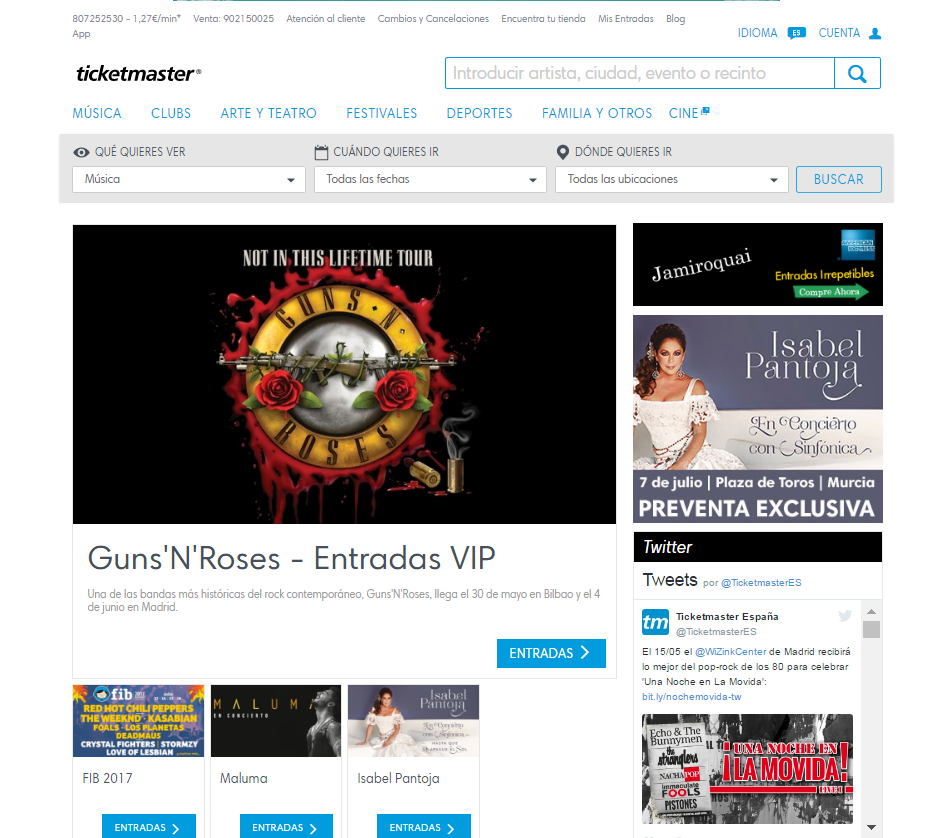
\includegraphics[width=0.42\linewidth]{Figures/EjemploWeb}}\hspace{1mm}
\subfigure[Pagina Entradas.com]{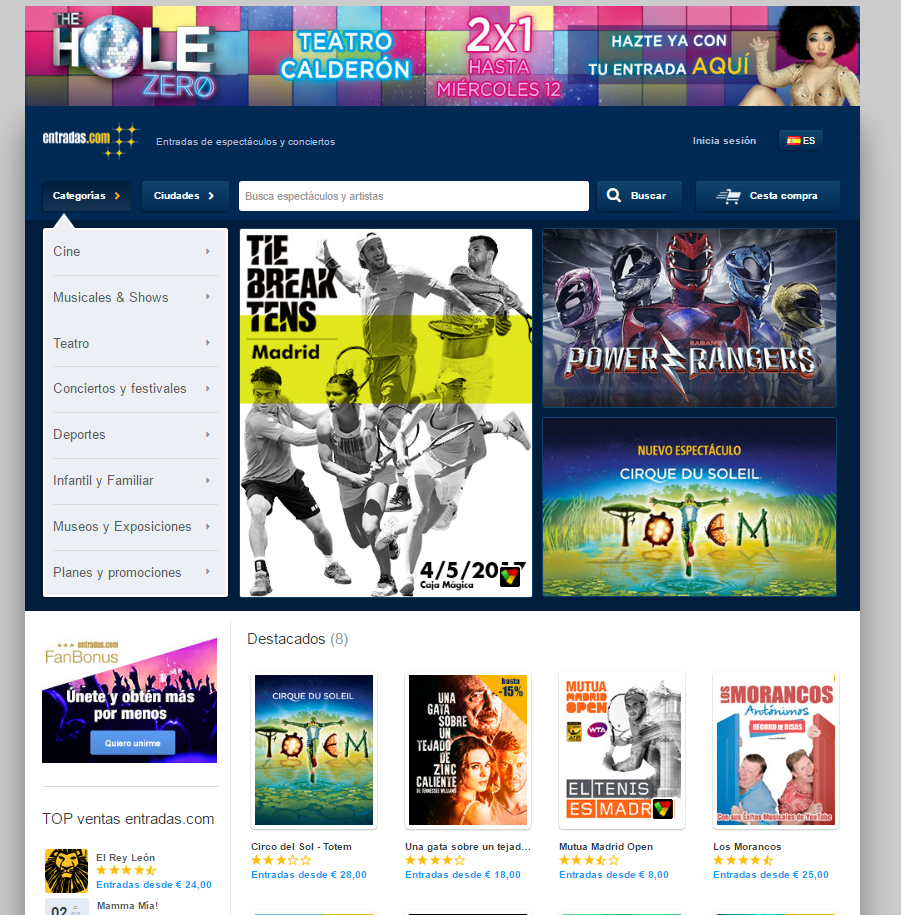
\includegraphics[width=0.42\linewidth]{Figures/EjemploWeb_2}}
\caption{Portada Paginas Web.}
\label{fig:Portadas_Web.}
\end{figure}
\\Por ello, en esta tercera practica se pide desarrollar un sitio web Full-Stack,es decir, nos encargamos de crear la capa Front-End y Back-End del proyecto y conocer como interactúan entre si estas dos capas.
\paragraph{Funcionalidad}
Para gestionar el contenido de la Web sera necesario implementar como BBDD MySQL. Además los usuarios tienen que tener acceso a los siguientes servicios de la aplicación y hacer uso de elementos multimedia (imágenes,audio y vídeo) para enriquecer la aplicación:
\begin{enumerate}
  \item \textbf{Cantantes:} Se muestra información ,vídeo,discos e imágenes del cantante.
  \item \textbf{Eventos:} Muestra información,localización,cantantes y entradas del evento.
\end{enumerate}
Por otra parte tiene que ser capas de gestionar los usuarios por medio de las siguientes funciones:
\begin{enumerate}
  \item \textbf{Register:} Entrega un formulario al usuario para registrarse en la aplicación.
  \item \textbf{Login:} Permite acceder al cliente siempre que se valide el contenido que rellene en el formulario de Login.
  \item \textbf{Perfil Usuario:} Disponible para aquellos usuarios que hayan realizado el Login y debe mostrar la información que el usuario a rellenado en la etapa de registro y un historial de las compras realizadas.
  \item \textbf{Logout:} Permite cerrar la sesión actual del usuario.
\end{enumerate}
Por ultimo,es necesario proveer a la aplicación de un carrito de la compra basado en la sesión del usuario con el objetivo de tener un mecanismo de persistencia permitiendo realizar las siguientes acciones:
\begin{enumerate}
  \item \textbf{Detalle del contenido:} Debe mostrar el contenido del carrito en una ventana individual  donde se detalla cada uno de los productos.
  \item \textbf{Actualizar contenido:} Se debe permitir la modificación del numero de productos añadidos.
  \item \textbf{Eliminar contenido:} Se debe permitir eliminar un producto que seleccione el cliente.
\end{enumerate}
\paragraph{Apariencia}
Al tratarse de un sitio Web es necesario darle un aspecto ordenado y cuidado aparte de las funcionalidad que se ha descrito por lo que se recomienda utilizar la librería de Boostrap.
\paragraph{Tecnologías Necesarias}
En el desarrollo de la practica es necesario/obligatorio que se haga uso de las tecnologías que se listan a continuación:
\begin{enumerate}
\item FrameWork:Django.
\item BBDD : MySQL.
\item Comunicación cliente-servidor(síncrono) : Formularios.
\item Comunicación cliente-servidor(asíncrono) : Ajax.
\item WebServices : Google Maps.
\item Mapas Interactivos : Google Maps (JS)
\item Boostrap
\end{enumerate}.
\section{Desarrollo Back-End}
Esta capa se encarga de buscar información en la BBDD de acuerdo a las peticiones que recibe y de entregar la información a los ficheros html correspondientes para que el navegador se encargue de cargarlos.
\\Primer vamos a instalar los controladores de MySQL que permiten a Django acceder al contenido de la BBDD así que a través de una consola ejecutamos los siguientes comandos:
\begin{enumerate}
\item \textbf{\textit{sudo apt -get install python-dev}}
\item \textbf{\textit{sudo apt -get install libmysqlclient-dev}}
\item \textbf{\textit{pip install MySQL-python}}
\end{enumerate}
El siguiente paso es crear la BBDD por lo que accedemos al promp de MySQL y ejecutamos \textit{\textbf{create database AppBBDD}}.Para comprobar que la BBDD se ha creado correctamente ejecutamos \textbf{\textit{show databases}} y veríamos algo parecido a la figura \ref{fig:Creacion_BBDD_APP}.
\begin{figure}[!h]
\begin{center}
   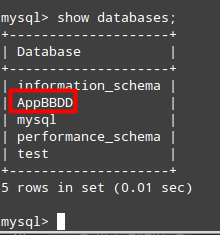
\includegraphics[width=0.2\linewidth]{Figures/Create_Databases}
  \decoRule
  \caption[Create BBDD]{Creación de la BBDD.}
\label{fig:Creacion_BBDD_APP}
\end{center}
\end{figure}
\\Tras terminar la configuración previa de componentes externos a Django es momento de trabajar con sus componentes internos que explicamos a continuación.
\subsection*{Conexión Django-BBDD}
La BBDD generada es AppBBDD que se incluye dentro del fichero \textbf{setting.py},permitiendo de esta forma acceder a la BBDD.
\begin{lstlisting}[
language=Python,
caption= añadimos la BBDD al entorno de Django.]
DATABASES = {'default': {
 'ENGINE': 'django.db.backends.mysql',
 'NAME': 'appBBDD',
 'USER':'root',
 'PASSWORD':'*******',
}
\end{lstlisting}
\subsection*{Modelos}
Hasta el momento solo se ha declaro la BBDD pero es necesario crear las tablas de la aplicación. La figura \ref{fig:Diagrama_modelos} describe el contenido de los modelos \footnote{https://github.com/RoboticsURJC-students/2015-TFG-Walter-Cuenca} diseñados y la su relación.
\begin{figure}[!h]
\begin{center}
   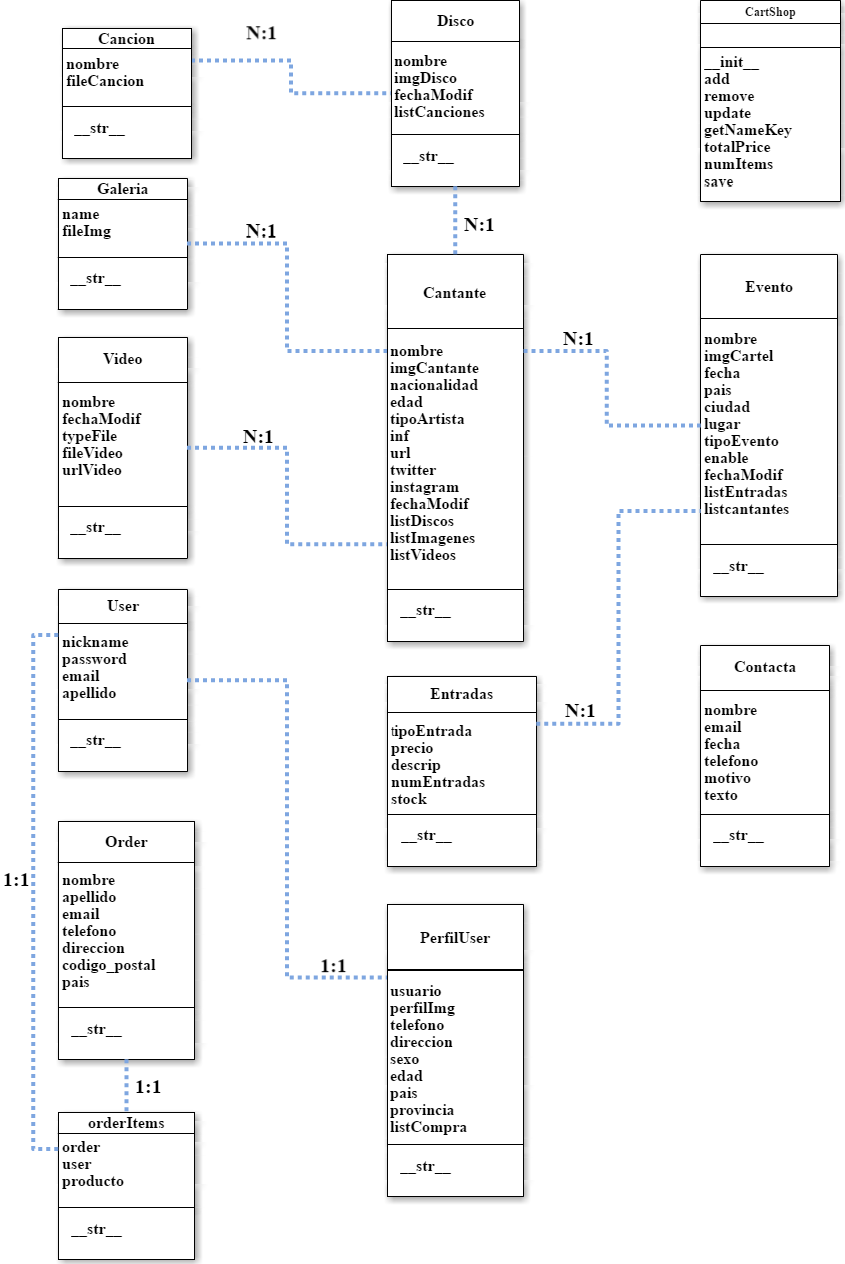
\includegraphics[width=0.45\linewidth]{Figures/Diagrama_modelos}
  \decoRule
  \caption[Diagrama modelos App.]{Diagrama modelos App.}
\label{fig:Diagrama_modelos}
\end{center}
\end{figure}
\\Para incluir información dentro de los modelos disponemos del interfaz admin de Django el cual abstrae la BBDD utiliza ademas de proporcionar un metodo mas amigable para el usuario. Se accede por medio de la url \textit{\textbf{128.0.0.1:/WebMultimedia/admin/}}, donde se visualizan los modelos incluidos en el fichero \textbf{admin.py}, figura \ref{fig:Admin_Django}.
\begin{figure}[!h]
\begin{center}
   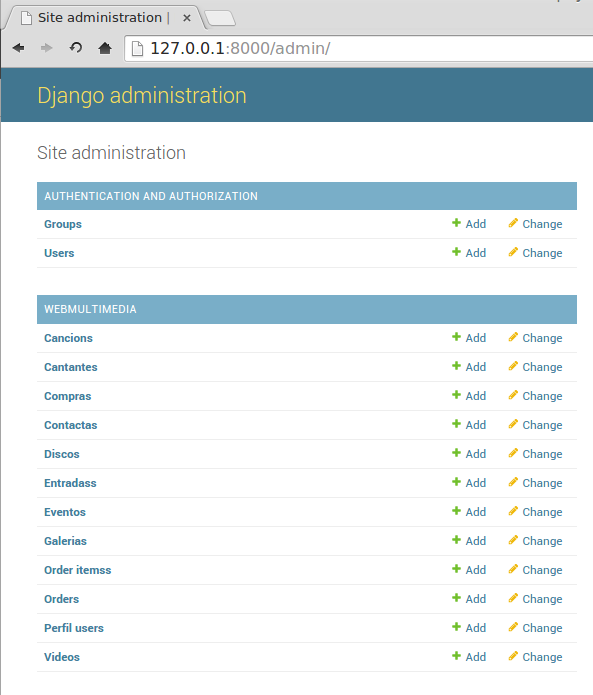
\includegraphics[width=0.3\linewidth]{Figures/admin_importModels}
  \decoRule
  \caption[Interfaz admin Django]{Interfaz admin Django}
\label{fig:Admin_Django}
\end{center}
\end{figure}
\subsection*{Formularios}
Generamos un fichero forms.py con varias clases que corresponden a los formulario de la aplicación. El objetivo de los formularios es recolectar información proporcionada por los usuarios y validarla una vez lleguen al servidor.
\begin{figure}[!h]
\begin{center}
   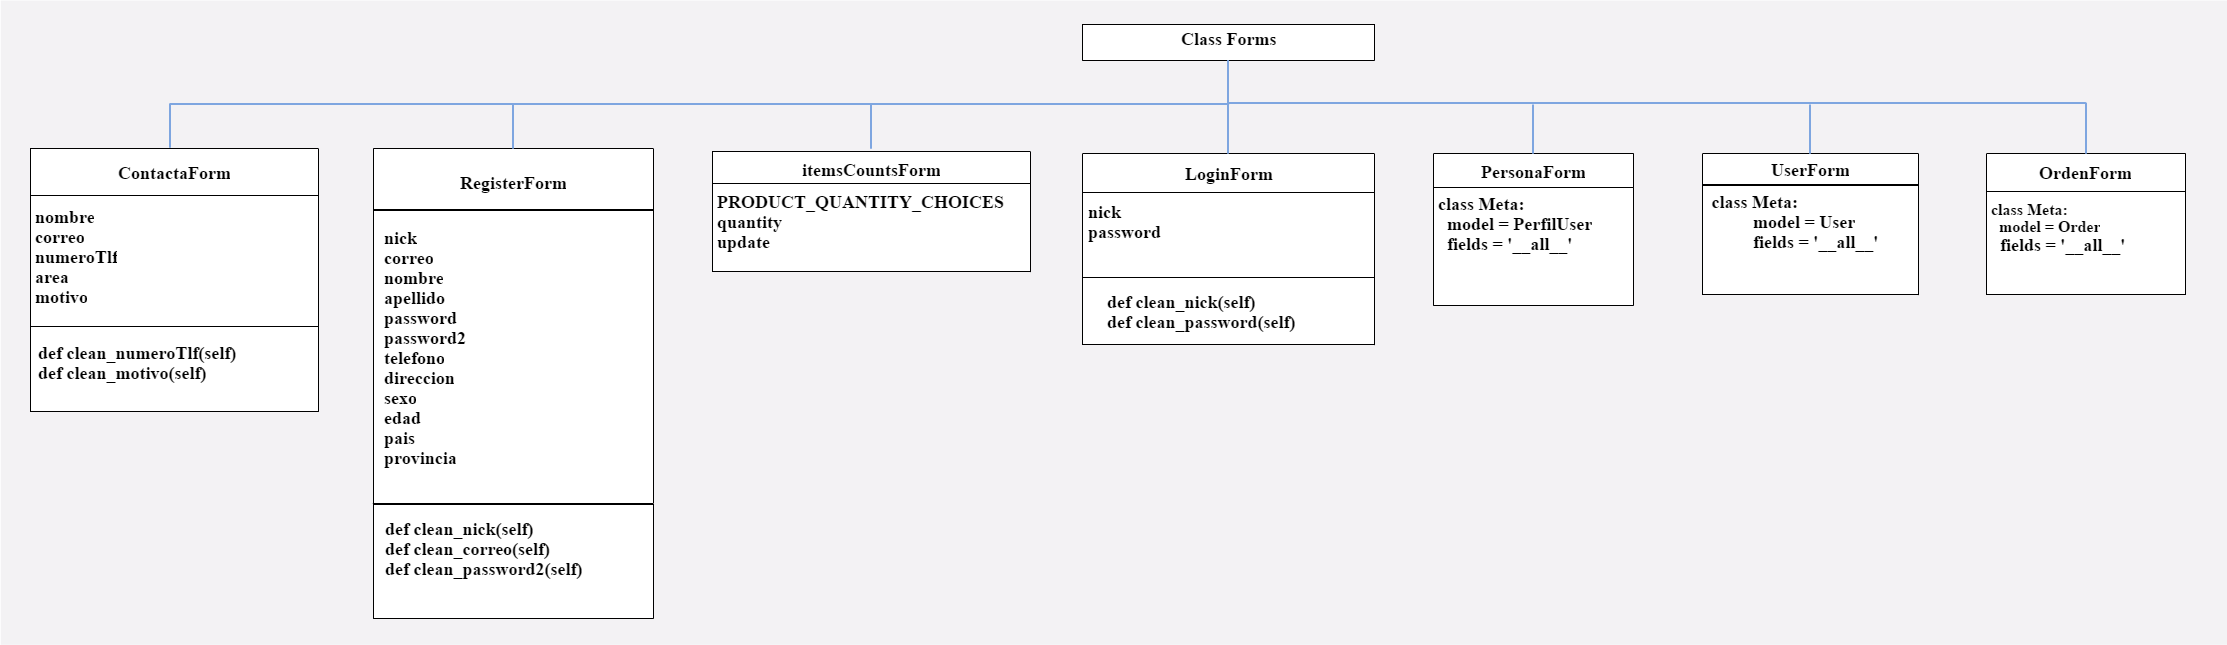
\includegraphics[width=1\linewidth]{Figures/diagrama_formularios}
  \decoRule
  \caption[Diagrama formularios de la aplicación.]{Diagrama formularios de la aplicación.}
\label{fig:diagrama_formularios}
\end{center}
\end{figure}
\subsection*{URL's}
Pasamos a definir las distintas URLs de la aplicación para permitir el acceso a los usuarios. La figura \ref{fig:Diagrama_URLs} muestra las características que tiene cada URL así como la vista que para trata cada la petición.
\begin{figure}[!h]
\begin{center}
   \includegraphics[width=0.6\linewidth]{Figures/Diagrama_URLs}
  \decoRule
  \caption[Diagrama URLs de la aplicación.]{Diagrama URLs de la aplicación.}
\label{fig:Diagrama_URLs}
\end{center}
\end{figure}
\subsection*{Vistas}
Pasamos a detallar el ultimo componente de esta capa que se encarga de interactuar con la BBDD obteniendo y/o guardando información recibida al acceder a las distintas URLs de la aplicación. La figura \ref{fig:diagrama_vistas} muestra las distintas vistas empleadas así como el parámetro que reciben en los casos que correspondan.
\begin{figure}[!h]
\begin{center}
   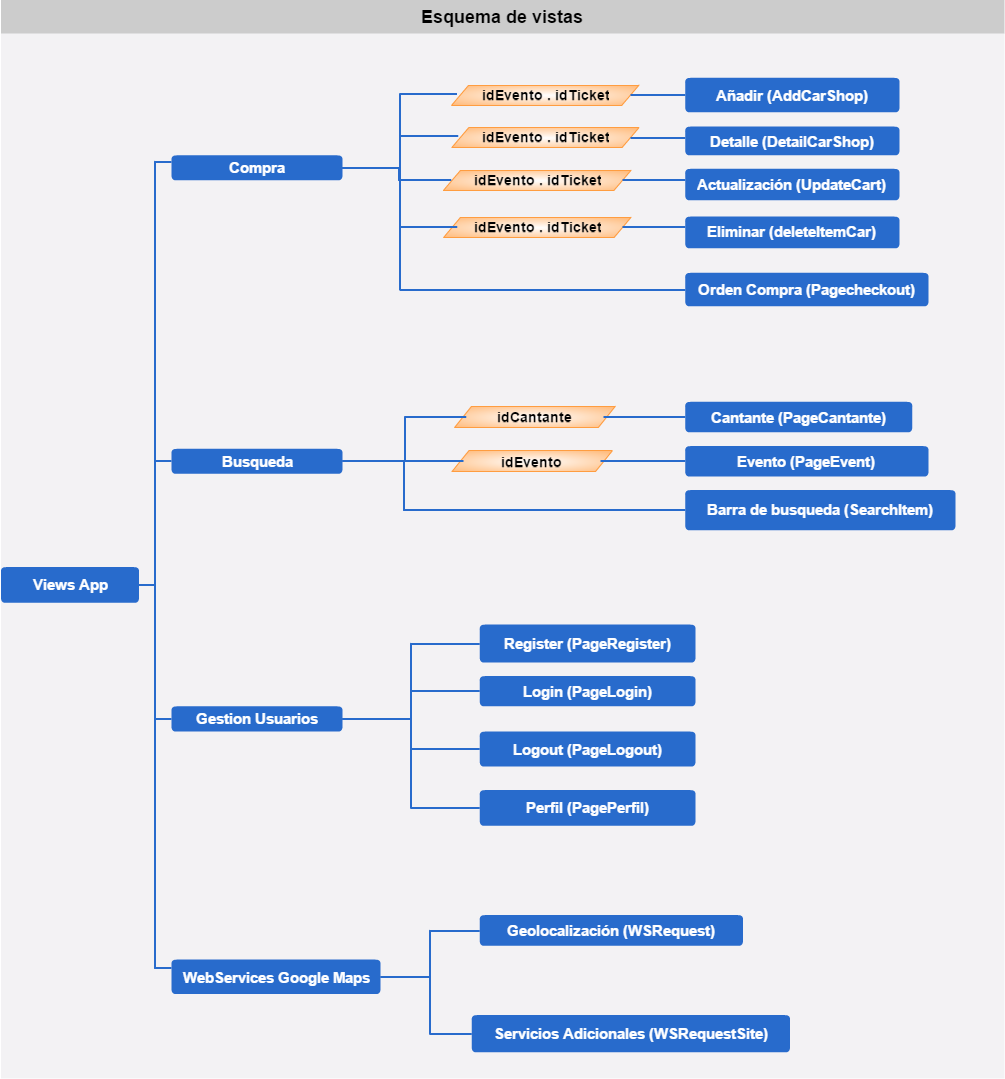
\includegraphics[width=0.7\linewidth]{Figures/diagrama_vistas}
  \decoRule
  \caption[Diagrama vistas de la aplicación.]{Diagrama vistas de la aplicación.}
\label{fig:diagrama_vistas}
\end{center}
\end{figure}
\\Las vistas utilizadas se han agrupado en cinco grupos según su funcionalidad, a continuación explicamos cada uno de ellos.
\begin{enumerate}
\item \textbf{Home:} Se encarga de obtener los cantantes y eventos que se han incluido en la BBDD en los últimos 15 días.
\item \textbf{Búsqueda:} Se encargan de buscar un determinado elemento en la BBDD como puede ser un Cantante,Evento o algún elemento de introducido por medio de la barra de búsqueda.
\item \textbf{Gestión de Usuarios:} Se encargan de gestionar el registro, login,logout o el perfil de un determinado usuario.
\item \textbf{Web Services Google:} Se encargan de gestionar peticiones al WebServices de Google Maps sobre la geolocalización de un lugar y servicios cercanos.
\end{enumerate}
\section{Desarrollo Front-End}
Esta capa de la aplicación se encarga del diseño de los ficheros html donde se vuelca la información de las vistas. Para acceder a la información es necesario aplicar el lenguaje de plantillas de Django.
\\La figura \ref{fig:diagrama_Front_End} muestra cada uno de los ficheros creados para la aplicación tanto html como js.
\begin{figure}[!h]
\begin{center}
   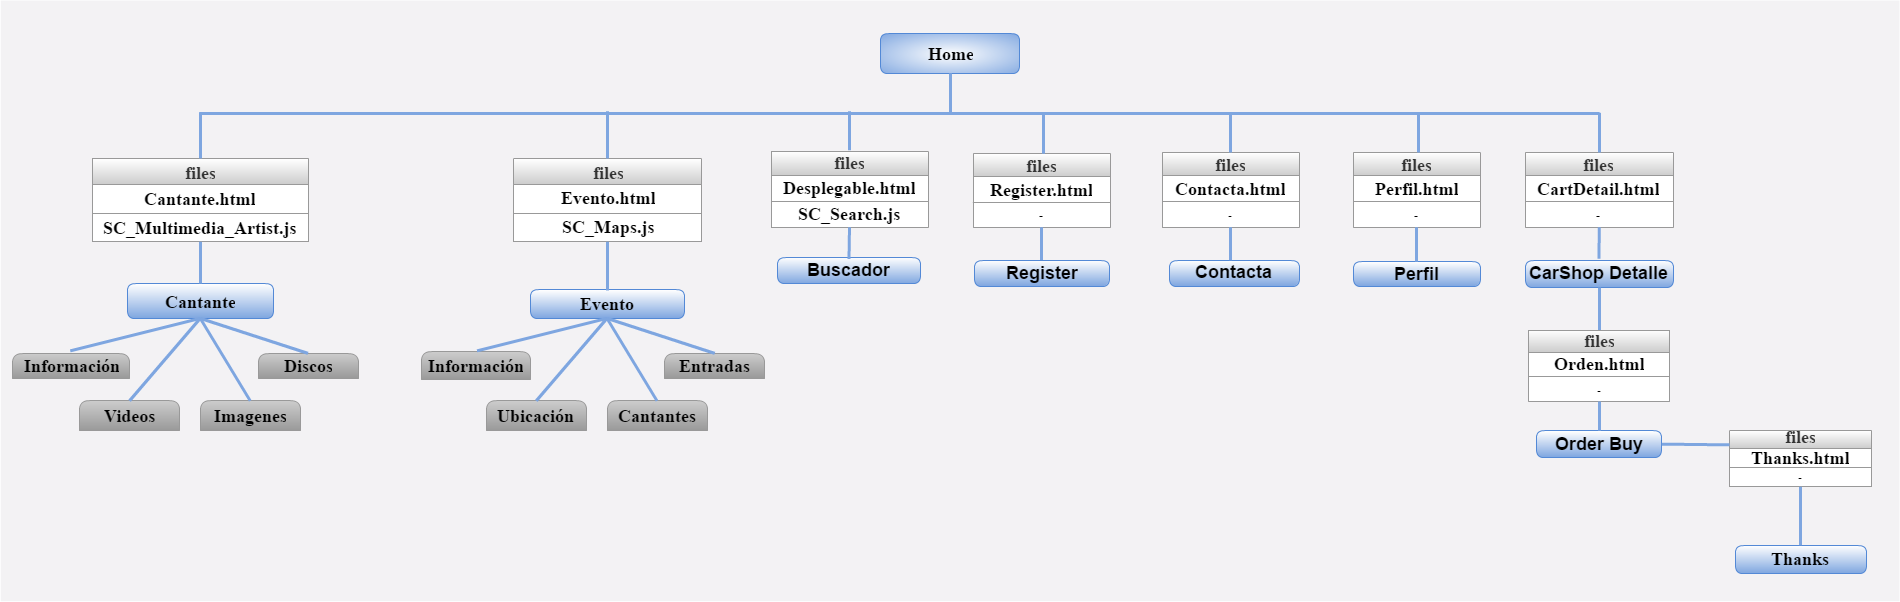
\includegraphics[width=0.8\linewidth]{Figures/diagrama_Front_End}
  \decoRule
  \caption[Diagrama ficheros Front-End de la aplicación.]{Diagrama ficheros Front-End de la aplicación.}
\label{fig:diagrama_Front_End}
\end{center}
\end{figure}
\\Ahora pasamos a explicar el contenido de cada uno de los ficheros tanto la apariencia como la funcionalidad.
\subsection*{Barra de Navegación}
Es el elemento principal de la aplicación donde se encuentran los accesos a las ventanas de la aplicación. La figura \ref{fig:Nav_Bar} muestra la apariencia de este elemento así como los distintos accesos.
\begin{figure}[!h]
\begin{center}
   
\includegraphics[width=0.7\linewidth]{Figures/Nav}
  \decoRule
  \caption[Barra de navegación]{Barra de navegación.}
\label{fig:Nav_Bar}
\end{center}
\end{figure}
\\En las siguientes subsecciones se muestra el aspecto y funcionalidad en el caso que corresponda de los distintos accesos.
\subsubsection*{Buscador}
Permite a los usuarios buscar cantantes o eventos introduciendo el nombre en el buscador obteniendo como resultado un desplegable. La figura \ref{fig:Search_Bar} muestra la apariencia.
\begin{figure}[!h]
\begin{center}
   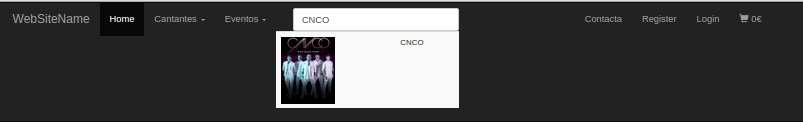
\includegraphics[width=0.7\linewidth]{Figures/Bar_Navegacion}
  \decoRule
  \caption[Buscador de la aplicación]{Buscador de la aplicación.}
\label{fig:Search_Bar}
\end{center}
\end{figure}
\\\underline{\textbf{Funcionalidad:}} La función \textbf{sendInfo()} recupera la información introducida por el usuario y valida su longitud ya que tiene que ser mayor a dos caracteres. Tras la validación realizamos una llamada Ajax a la url \textit{\textbf{/WebMutimedia/Search/}} por medio de la función \textbf{AjaxRequest(data)}.
\begin{lstlisting}[
caption=Petición Ajax buscador aplicación.]
function sendInfo(){
  texto = $('#textSearch').val();
  console.log(texto);
  if(texto.length > 2){
    AjaxRequest(texto);
  }else{
    $("table#tbSearch").remove();
  }
}

function AjaxRequest(data){
  $.ajax({ 
    type: "POST",
    url:'/WebMutimedia/Search/',
    data: {
      'textRequest' : data,
      'csrfmiddlewaretoken': $("input[name=csrfmiddlewaretoken]").val(),
    },
    success: resulSearch,
    dataType: 'html',
  });
}
\end{lstlisting}
La función \textbf{resulSearch()} definida en la petición se encarga de recibir la respuesta e insertarla en la pagina.
\begin{lstlisting}[
caption=Respuesta Ajax buscador aplicación.]
function resulSearch(data, textStatus, jqXHR){
    $('#listSearch').html(data);
}
\end{lstlisting}
\subsubsection*{Contacta}
Al acceder al enlace se redirecciona al usuario a la url \textbf{\textit{/WebMutimedia/Contacta}} obteniendo como resultado un formulario del contacta como se ve en la figura \ref{fig:Form_Contacta}.
\begin{figure}[!h]
\begin{center}
   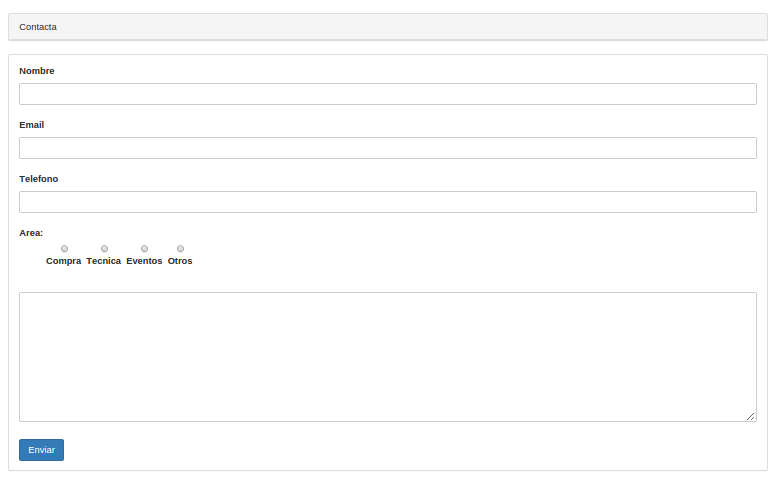
\includegraphics[width=0.7\linewidth]{Figures/Contacta}
  \decoRule
  \caption[Pagina Contacta]{Pagina Contacta.}
\label{fig:Form_Contacta}
\end{center}
\end{figure}
\subsubsection*{Register}
Al acceder al enlace se redirecciona al usuario a la url \textbf{\textit{/WebMutimedia/Register}} obteniendo como resultado el formulario de registro como se ve en la figura \ref{fig:Form_Register}.
\begin{figure}[!h]
\begin{center}
  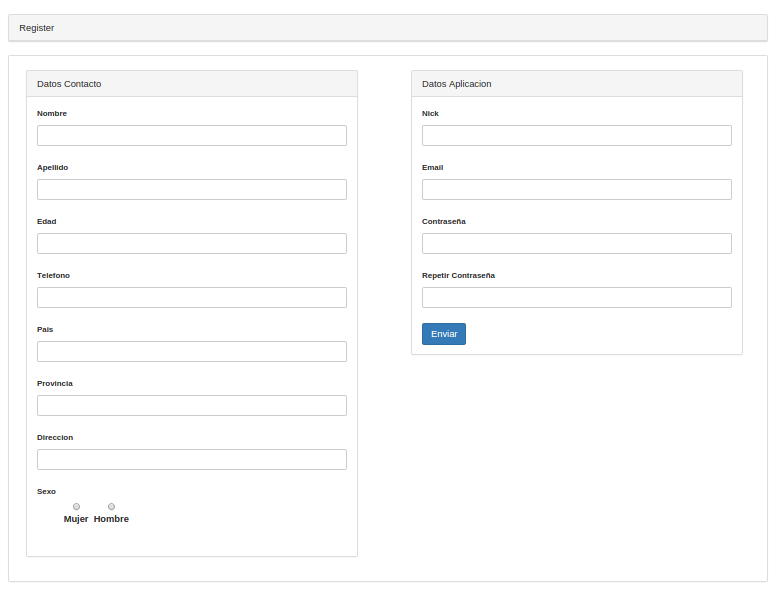
\includegraphics[width=0.7\linewidth]{Figures/Register}
  \decoRule
  \caption[Pagina Registro]{Pagina Registro.}
\label{fig:Form_Register}
\end{center}
\end{figure}
\subsubsection*{Login}
Al pulsar el enlace se activa el formulario de la figura\ref{fig:Form_Login} que contiene como campos el nombre del usuario y password que se enviara a la url\textit{\textbf{ /WebMultimedia/Login}}.
\begin{figure}[!h]
\begin{center}
   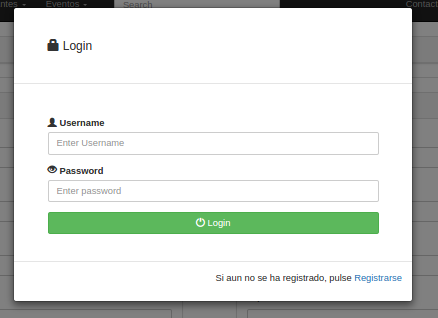
\includegraphics[width=0.4\linewidth]{Figures/Login}
  \decoRule
  \caption[Formulario Login]{Formulario Login.}
\label{fig:Form_Login}
\end{center}
\end{figure}
\subsubsection*{Perfil}
Al pulsar el enlace se redirecciona a la url \textbf{\textit{/WebMutimedia/Perfil}} obtiendo como resultado la figura \ref{fig:Perfil_user} donde se muestra la información del usuario y las compras realizadas en la aplicación.
\begin{figure}[!h]
\begin{center}
   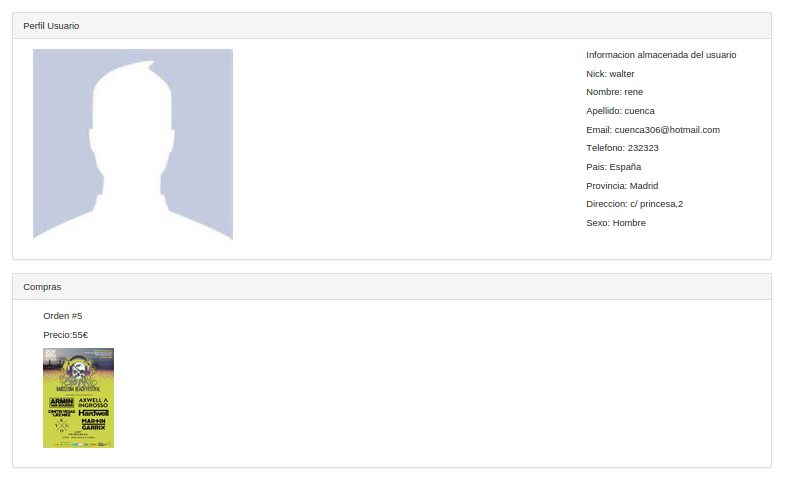
\includegraphics[width=0.6\linewidth]{Figures/ProfileUser}
  \decoRule
  \caption[Perfil Usuario]{Pagina Perfil Usuario.}
\label{fig:Perfil_user}
\end{center}
\end{figure}
\subsubsection*{Logout}
Al acceder a este enlace se redirecciona a la url \textbf{\textit{'/WebMultimedia/Logout'}} que finaliza la sesión del usuario.
\subsection*{Home}
La pagina principal de la aplicación se obtiene al acceder a la url \textit{\textbf{ '/WebMultimedia/'}} que muestra consta de un carrusel de imágenes y una sección de novedades de cantantes y eventos como se ve en la figura \ref{fig:Page_Home}.
\begin{figure}[!h]
\begin{center}
   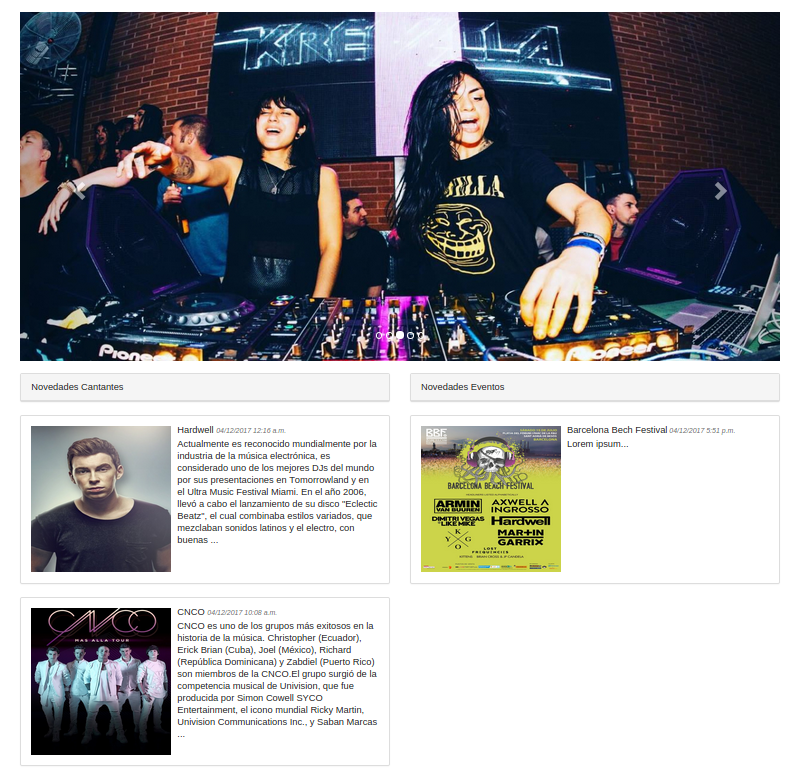
\includegraphics[width=0.5\linewidth]{Figures/HomePage}
  \decoRule
  \caption[Pagina Principal]{Pagina Principal.}
\label{fig:Page_Home}
\end{center}
\end{figure}
\subsection*{Cantantes} 
El usuario selecciona un cantante del desplegable provocando la redireccion a la url \textit{\textbf{'/WebMultimedia/Cantante/idCantante/'}} que muestra la información del cantante que se distribuye en cuatro tabs que pasamos a explicar.
\subsubsection*{Información}
Contiene información del cantante además de su foto como se ve en la figura \ref{fig:Info_Cantante}.
\begin{figure}[!h]
\begin{center}
   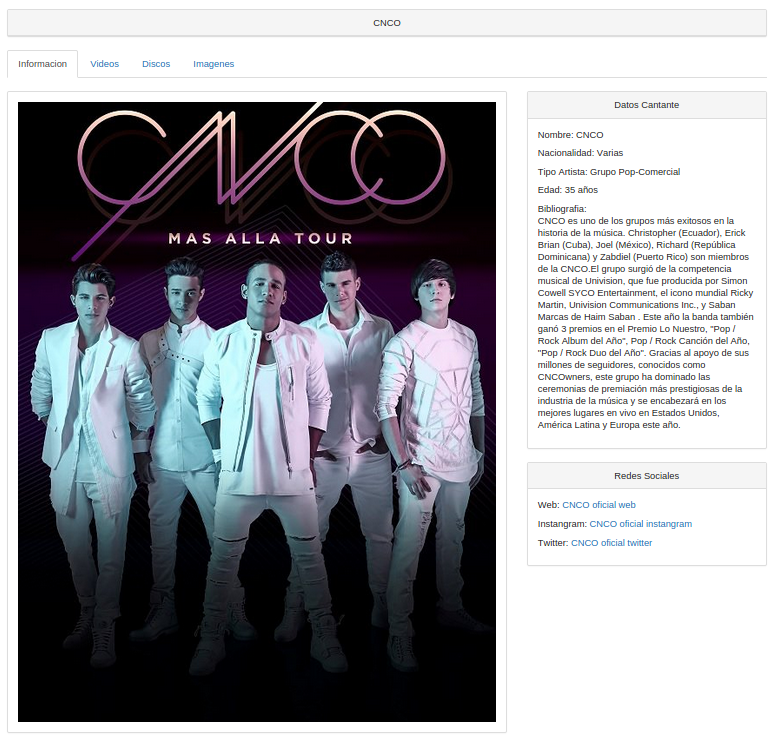
\includegraphics[width=0.45\linewidth]{Figures/init_Cantante}
  \decoRule
  \caption[Cantante panel Información]{Pagina Cantante panel Información.}
\label{fig:Info_Cantante}
\end{center}
\end{figure}
\subsubsection*{Vídeos}
Contiene una lista con los vídeos de los que dispone la aplicación sobre el cantante como muestra la figura \ref{fig:Video_Cantante}.
\begin{figure}[!h]
\begin{center}
   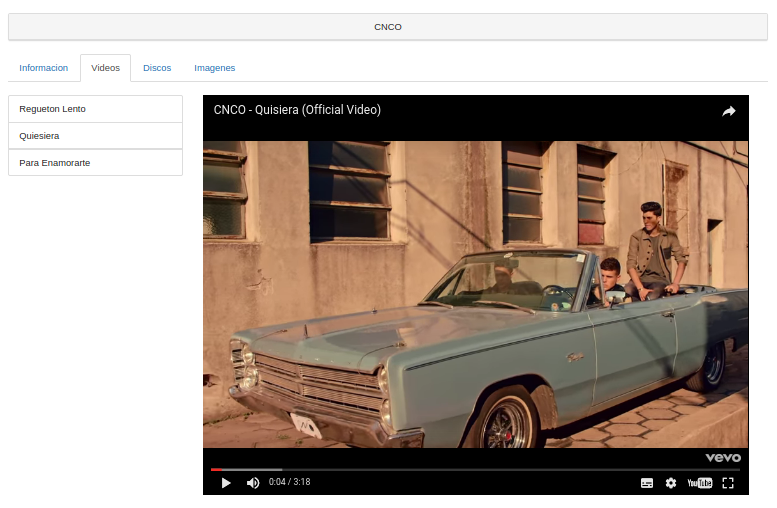
\includegraphics[width=0.45\linewidth]{Figures/videos_Cantante}
  \decoRule
  \caption[Cantante panel Información]{Pagina Cantante panel Información.}
\label{fig:Video_Cantante}
\end{center}
\end{figure}
\\\underline{\textbf{Funcionalidad:}} Para permitir que los usuarios seleccionen un vídeo de la lista creamos la función \textit{\textbf{'loadVideo(file,tipo)'}} y lo vinculamos a cada uno de los elementos.
\\La función evalúa el tipo de archivo del que se trata ya que puede ser \textbf{<iframe>} o \textbf{<video>} y así reproducirlo a través del elemento adecuado.
\begin{lstlisting}[
caption=Función carga de vídeos.]
 function loadVideo(file,tipo){
  if(tipo == 'iframe'){
   $('iframe').attr("src",file);
   $("video").hide();
   $("iframe").show();
  }else{
   var path ='/media/'+file;
   $('video').attr("src",path);
   $("iframe").hide();
   $("video").show();
  }
 }
\end{lstlisting}
\subsubsection*{Discos}
Contiene los discos relacionados con el cantante además de una lista de reproducción para escuchar las canciones de un disco tras ser seleccionado. La apariencia se muestra en la figura \ref{fig:Discos_Cantante}.
\begin{figure}[!h]
\begin{center}
   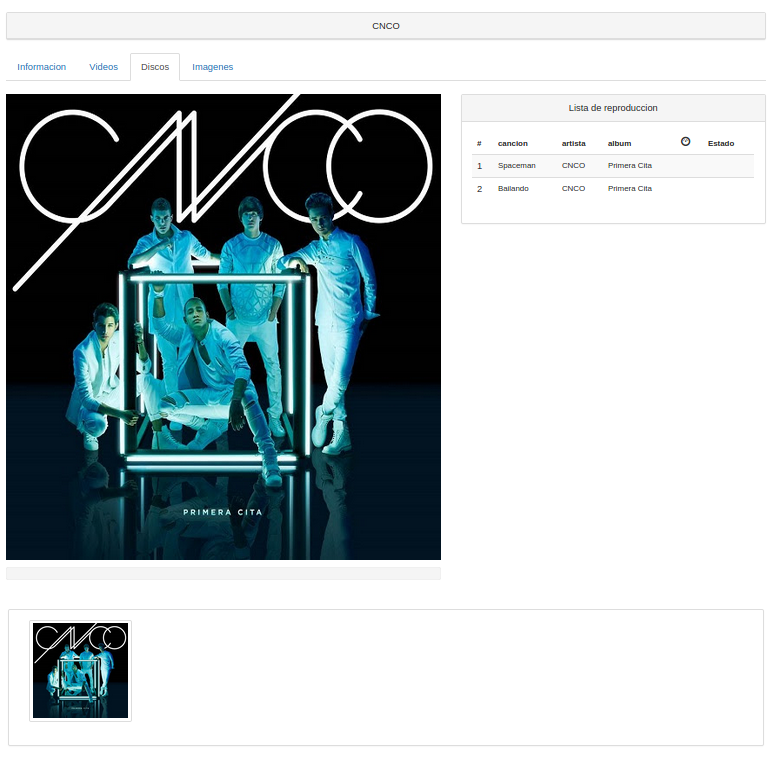
\includegraphics[width=0.4\linewidth]{Figures/discos_Cantante}
  \decoRule
  \caption[Cantante panel Discos]{Pagina Cantante panel Discos.}
\label{fig:Discos_Cantante}
\end{center}
\end{figure}
\\\underline{\textbf{Funcionalidad:}} Los usuarios al seleccionar provoca la llamada a la función \textbf{loadList)}. La función carga la imagen del disco y las canciones en la lista de reproducción.
\begin{lstlisting}[
language=JavaScript,
caption=Función carga lista de reproducción.]
function loadList(elemente,imagen){
 $('#ImgRepro').attr('src','/media/'+imagen);
 var idElemento = $(elemente).attr("id");
 var divListSong = $('#'+idElemento).siblings('div');
 var idDivListSong = $(divListSong).attr("id");
 $("table#x").remove();
 $('#'+idDivListSong).children('table').clone().appendTo($('#x'));
}
\end{lstlisting}
Para reproducir una canción de la lista se emplea la función \textbf{loadSong()}. La función se encarga de obtener el elemento a reproducir al igual que el tiempo duración en la lista de producción.
\begin{lstlisting}[
caption=Función reproducir canción.]
 function loadSong(name,idElement,urlSong){
  var idTimer = 'timer_'+idElement;
  var state_Actual = 'state_'+idElement;
  var path = '/media/'+urlSong;
  var audio = document.getElementById('repro');
  if(!audio.paused){
   audio.pause();
  }
  if (state_Actual != stado_Old && stado_Old != ''){
   document.getElementById(stado_Old).innerHTML = '';
  }
  audio.src = path; 
  audio.onloadeddata=function() {
   var str_Time = convertSeg_Min(audio.duration);
   document.getElementById(state_Actual).innerHTML = 'Reproduciendo';
   document.getElementById(idTimer).innerHTML = str_Time;
   audio.play();
   stado_Old = state_Actual;
  }
 }
\end{lstlisting}
\subsubsection*{Imágenes}
Contiene un conjunto de imágenes en forma de galeria como se ve en la figura \ref{fig:Imagenes_Cantante}.
\begin{figure}[!h]
\begin{center}
   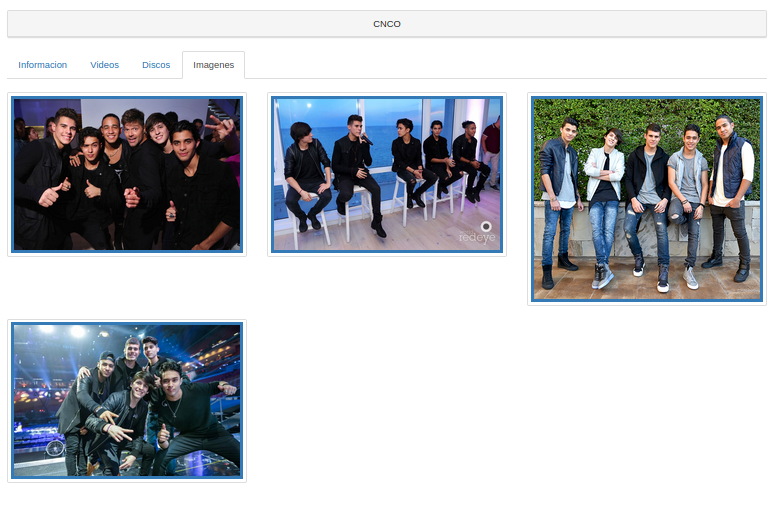
\includegraphics[width=0.5\linewidth]{Figures/imagenes_Cantante}
  \decoRule
  \caption[Cantante pestaña imágenes]{Pagina Cantante pestaña imágenes.}
\label{fig:Imagenes_Cantante}
\end{center}
\end{figure}
\subsection*{Eventos}
Al seleccionar un evento del desplegable redirecciona al usuario a la url \textit{\textbf{'/WebMultimedia/Eventos/idvento/'}} que muestra la información en cuatro paneles que pasamos a explicar.
\subsubsection*{1. Información}
Este panel contiene varia información sobre el evento como se ve en la figura \ref{fig:Informacion_Evento}.
\begin{figure}[!h]
\begin{center}
   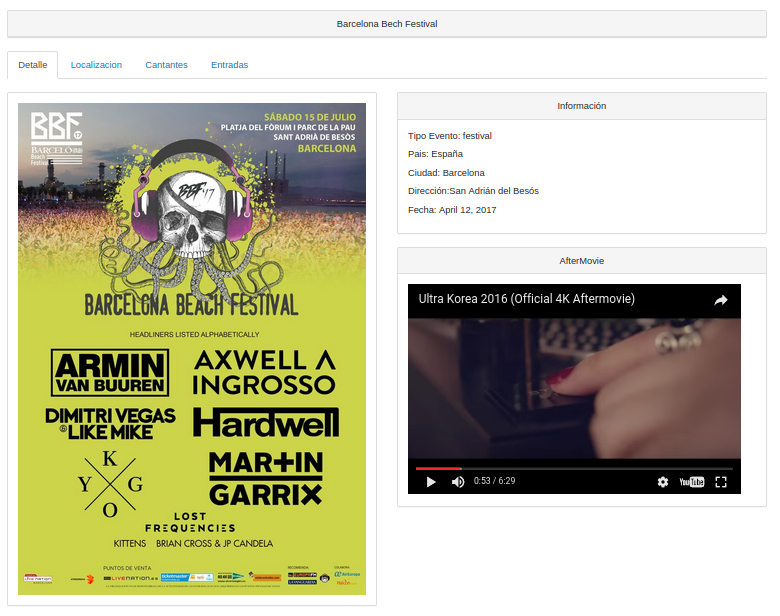
\includegraphics[width=0.5\linewidth]{Figures/Init_Evento}
  \decoRule
  \caption[Evento panel Información]{Pagina Evento panel Información.}
\label{fig:Informacion_Evento}
\end{center}
\end{figure}
\subsubsection*{2. Ubicación}
 Muestra la ubicación del evento y los servicios(hoteles,restaurantes,...) alrededor del lugar en un mapa como se ve en la figura \ref{fig:Ubicacion_Evento}.
\begin{figure}[!h]
\begin{center}
   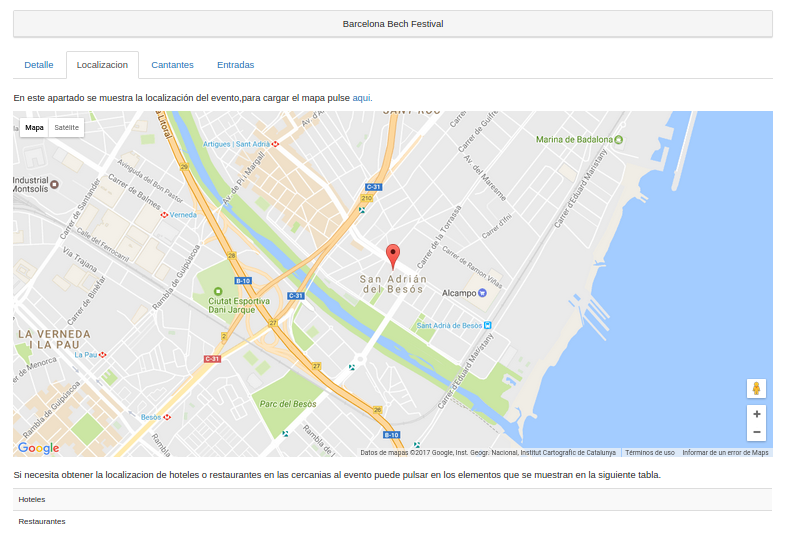
\includegraphics[width=0.6\linewidth]{Figures/Ubicacion_Evento}
  \decoRule
  \caption[ Evento panel ubicación]{Pagina Evento panel ubicación.}
\label{fig:Ubicacion_Evento}
\end{center}
\end{figure}
\\\underline{\textbf{Funcionalidad:}} Se realiza una llamada Ajax a la url \textit{\textbf{ "/WebMutimedia/WebServRequest/"}} con el nombre del lugar. Definimos la función \textit{\textbf{searchSucess}} para recuperar la respuesta del servidor.
\begin{lstlisting}[
language=JavaScript,
caption=Petición Ajax Ubicación Lugar.]
 $.ajax({ 
  type: "POST",
  url:"/WebMutimedia/WebServRequest/",
  data: {
   'site' :$('#direct').text(),
   'csrfmiddlewaretoken': $("input[name=csrfmiddlewaretoken]").val(),
  },
  success: searchSucess,
  dataType: 'html',
 });
\end{lstlisting}
La función \textbf{searchSucess} parsea a formato JSON el contiene de la variable \textbf{data} para obtener la información de las coordenadas accediendo a \textbf{geometry.location}.
\begin{lstlisting}[
caption=Respuesta Ajax Ubicación Lugar.]  
 function searchSucess(data, textStatus, jqXHR){
  var infoRequest = JSON.parse(data);
  coordenadas = infoRequest.results[0].geometry.location;
  WarchMap();  
 }
\end{lstlisting}
La función \textbf{ WarchMap()} se encarga de crear el mapa realizando una instancia de \textit{\textbf{google.maps.Map()}} que recibe como parámetro el lugar de la pagina donde se visualizara y sus propiedades que se definen en la variable \textbf{mapProp}. Finalmente con las coordenadas realiza una instancia de \textit{\textbf{google.maps.Marker}} asociándolo al mapa con el objetivo de indicar claramente el lugar del evento.
\begin{lstlisting}[
caption=Creación Mapa con la Ubicación.]
 function WarchMap(){
  var lat = parseFloat(coordenadas.lat);
  var long = parseFloat(coordenadas.lng);
  var mapProp = {
    center:new google.maps.LatLng(lat,long),
    zoom:15,
    mapTypeId:google.maps.MapTypeId.ROADMAP,
  };
  map=new google.maps.Map(document.getElementById("Maps"),mapProp);
  var marker = new google.maps.Marker({
   position: { lat:parseFloat(coordenadas.lat),lng:parseFloat(coordenadas.lng) },
   draggable: true,
   animation: google.maps.Animation.BOUNCE,
   map: map,
   title: 'Concierto'
  });
 }
\end{lstlisting}
\subsubsection*{3. Cantantes}
El panel contiene imágenes de los cantantes que tienen relación con el evento seleccionando como se puede ver en la figura \ref{fig:Cantantes_Evento}.
\begin{figure}[!h]
\begin{center}
   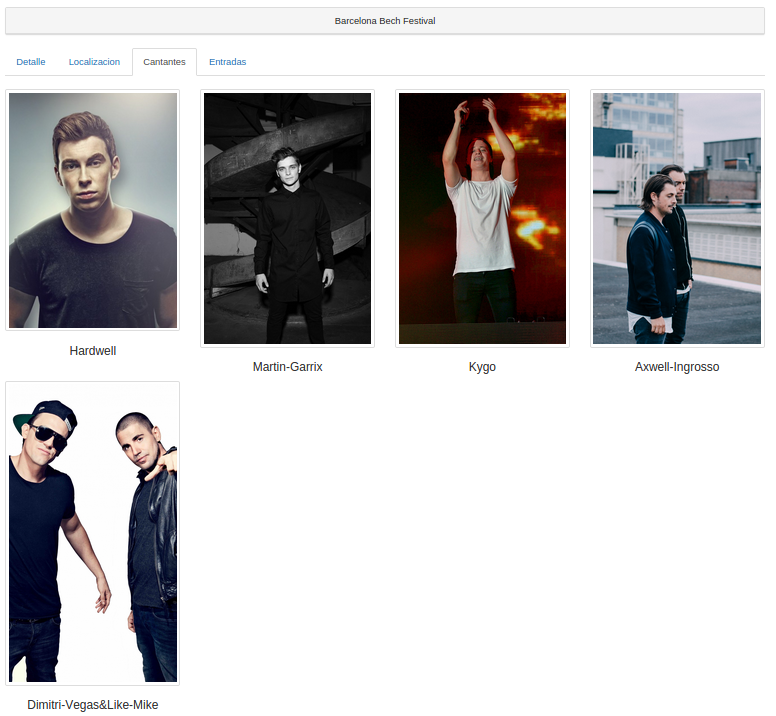
\includegraphics[width=0.5\linewidth]{Figures/Cantantes_Evento}
  \decoRule
  \caption[Evento panel Cantantes]{Pagina Evento panel Cantantes.}
\label{fig:Cantantes_Evento}
\end{center}
\end{figure}
\subsubsection*{4. Entradas}
El panel contiene las entradas de las que dispone el evento  además de una pequeña descripción como se puede ver en la figura \ref{fig:Entradas_Evento}.
\begin{figure}[!h]
\begin{center}
   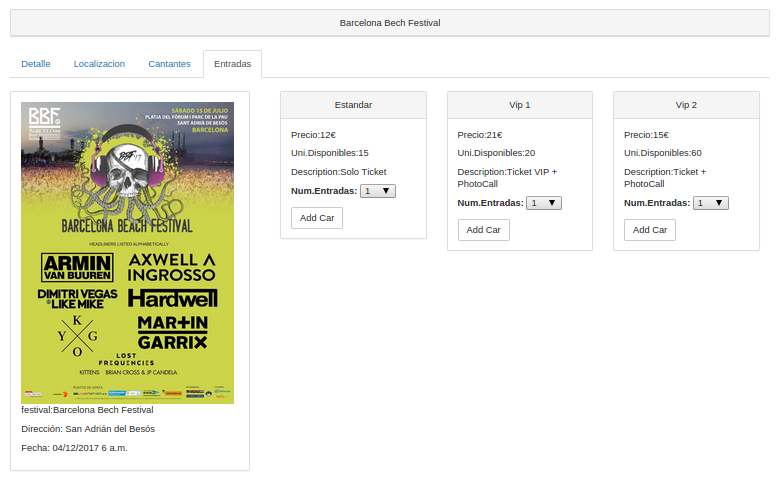
\includegraphics[width=0.5\linewidth]{Figures/Entradas_Evento}
  \decoRule
  \caption[Evento pestaña Entradas]{Pagina Evento pestaña Entradas.}
\label{fig:Entradas_Evento}
\end{center}
\end{figure}
\\\underline{\textbf{Funcionalidad:}} Los usuarios añaden contenido al carrito de la compra por medio del botón \textbf{Add Car} disponible en cada tipo de entrada que redirecciona a la url \textbf{\textit{/WebMutimedia/AddCar/{{evento.id}}/{{ticket.id}}}} provocando que se añade este elemento al carrito de la compra del usuario.
\subsection*{Carrito de la Compra}
Es necesario permitir a los usuarios visualizar el detalle de su compra por lo que al pulsar sobre el enlace de la barra de navegación accedemos a la url \textit{\textbf{'/WebMutimedia/DetailCar/'}} mostrando cada uno de los productos como se ve en la figura \ref{fig:Detalle_CarShop}. 
\begin{figure}[!h]
  \begin{center}
     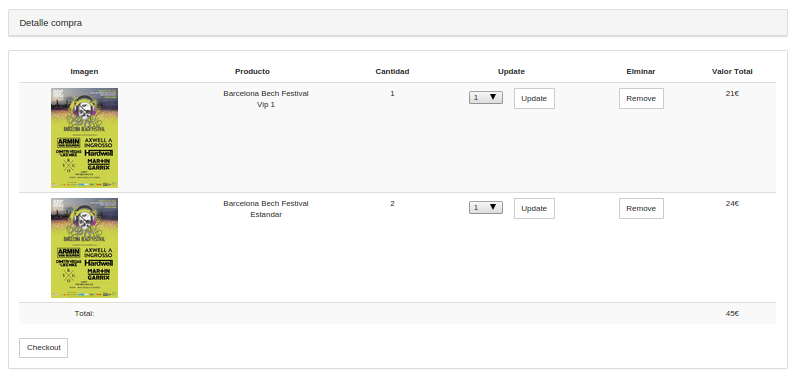
\includegraphics[width=0.8\linewidth]{Figures/Detalle_CarShop}
      \decoRule
      \caption[Detalle Carrito]{Pagina Detalle Carrito.}
  \label{fig:Detalle_CarShop}
  \end{center}
\end{figure}
\\\underline{\textbf{Funcionalidad:}}Dentro del detalle de la compra es necesario proveer de varias acciones que explicamos a continuación para que el usuario pueda realizar modificaciones del contenido de su carrito.
\begin{enumerate}
\item \textbf{Actualizar}: Al seleccionar un nuevo numero de entradas y pulsar \textbf{'Update'} se redirecciona la petición a la url \textit{\textbf{'WebMultimedi/UpdateCar/idEvento/idTicket/'}} que se encarga llevar acabo la acción.
\item \textbf{Eliminar}: Al pulsar \textbf{'Remove'} se redirecciona la petición a la url \textit{\textbf{'WebMultimedia/RemoveCart/idEvento/idTicket/'}}
\item \textbf{Checkout}: Permite pasar a tramitar la orden de compra de los producto redireccionando la acción a la url \textit{\textbf{'WebMultimedia/Checkout/'}}.
\end{enumerate}
\subsection*{Orden de Compra}
Esta ventana es visible cuando el usuario desea terminar la compra del contenido de su carrito  ya que muestra un resumen de los elementos añadidos y un formulario con los datos del usuario para generar la orden . El aspecto de esta pagina se muestra la figura  \ref{fig:Page_OrdenCompra}.
\begin{figure}[!h]
\begin{center}
   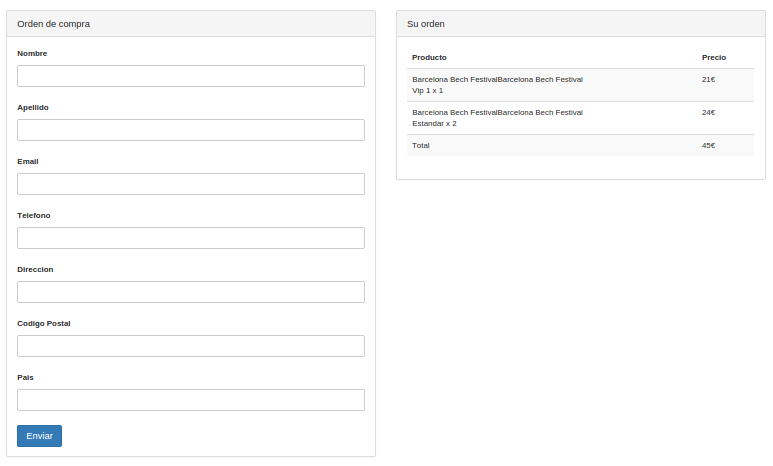
\includegraphics[width=0.5\linewidth]{Figures/CheckOut_CarShop}
  \decoRule
  \caption[ Orden Compra]{Pagina Orden Compra.}
\label{fig:Page_OrdenCompra}
\end{center}
\end{figure}
\section{Pruebas}